\documentclass[a4paper,11pt,fleqn]{article}%fleqn pour aligner les equations à gauche
\usepackage{../../Styles/Cours}

\newcommand{\chnum}{Chapitre 3}
\newcommand{\chtitle}{Évolution des quantités de matière pendant un titrage}
\newcommand{\dtype}{TP}


\begin{document}
\maketitle

Le vinaigre est une solution aqueuse d'acide éthanoïque (appelé aussi acide acétique) de formule \ce{CH3CO2H}. Ses propriétés acides en font un excellent anticalcaire, détartrant, désinfectant ou encore désodorisant. Il peut ainsi remplacer bon nombre de produits ménagers, comme les anticalcaires et antitartres, les produits pour laver les vitres ou pour récurer, l'assouplissant ...\\
\textbf{Problématique : Quelle est la concentration d'acide éthanoïque dans les vinaigre ?}
\section{Détermination expérimentale par titrage avec suivi pH-métrique}
\begin{figure}[h!]
	\begin{minipage}{.48\textwidth}
		\caption{\textbf{Titrage}}
    Lorsque l'espèce à titrer possède des propriétés acides, on la fait réagir avec une espèce titrante basique (et réciproquement). L'espèce à titrer étant progressivement consommée, le pH du milieu varie. \textbf{Le titrage par suivi pH-métrique consiste à suivre l'évolution de pH au fur et à mesure de l'ajout de solution titrante.} Cette évolution permet de repérer l'équivalence et ainsi de déterminer la quantité de matière ou la concentration initiale de l'espèce titrée.\\
    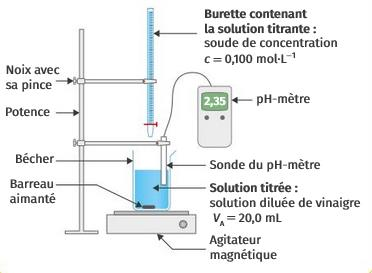
\includegraphics[scale=.55]{Ressources/TSPE_C3_AE_Fig1.png}
    \end{minipage}
 \begin{minipage}{.48\textwidth}
	\caption{\textbf{Matériel}}
	\begin{itemize*}
		\item 3 béchers
		\item une fiole jaugée de 50 mL et une de 100 mL
		\item une burette graduée de 25 mL
		\item des pipettes jaugées de 5 mL et de 20 mL
		\item une propipette ou une poire à pipeter
		\item une pipette pasteur + un petit bécher en plastique
		\item un agitateur magnétique (barreau aimanté au bureau)
		\item un pH-mètre
		\item du papier filtre
		\item un ordinateur équipé de \textit{Latis Pro}
		\item du vinaigre blanc à 8\%
		\item solution d'hydroxyde de sodium de concentration $c_B$ = \SI{1,00E-1}{\mole\per\liter}
		\item solution tampon de pH = 7 et pH = 4
		\item pissette d'eau distillée
	\end{itemize*}
 \end{minipage}
\end{figure}
\subsection*{S'approprier}
\begin{enumerate}
	\item \begin{enumerate}
		\item Montrer que l'acide éthanoïque est un acide au sens de Brönsted.
		\item Donner le couple acide/base auquel il appartient.
		\item Identifier le réactif titrant et donner le couple acide/base auquel il appartient.
		\item En déduire la réaction support du titrage.
	\end{enumerate}
	\item \begin{enumerate}
		\item Quelles sont les deux grandeurs que l'on mesure lors d'un titrage par suivi pH-métrique ?
		\item Prévoir de quelle manière va évoluer le ph au cours de cette transformation. Expliquer.
	\end{enumerate}
 \end{enumerate}

\subsection*{Réaliser}
\begin{enumerate}[resume]
	\item \begin{enumerate}
		\item Avant d'être dosé, le vinaigre commercial doit être dilué 20 fois. Proposer une explication.
		\item Choisir, parmi le matériel disponible, la verrerie utile pour réaliser cette dilution.
	\end{enumerate}
	\begin{tabular}{m{13cm} m{4cm}}
	\begin{itemize}
		\item Réaliser la dilution
		\item Étalonner le pH-mètre en suivant le mode opératoire indiqué sur la fiche
		\item Prélever \SI{20}{mL} de vinaigre dilué et les placer dans un bécher
		\item Rincer la burette avec la solution titrante, puis la remplir
		\item Mettre en place le montage de titrage
		\item Ajouter progressivement (voir la figure ci-contre) la solution titrante et noter la valeur du pH une fois stabilisé.
	\end{itemize} & 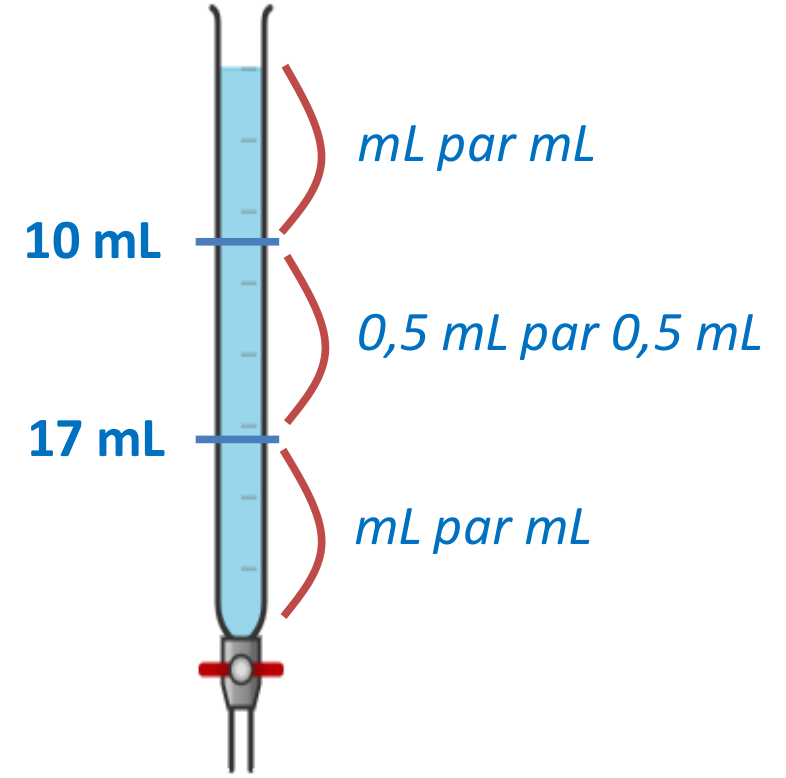
\includegraphics[scale=.17]{Ressources/TSPE_C3_AE_Fig2.png}\\
	\end{tabular}
	\item Décrire l'évolution du pH au cours de ce titrage. Est ce en accord avec les prévisions de la question 3 ?
\end{enumerate}
	L'équivalence intervient au milieu de la brusque variation de pH. On peut déterminer le milieu de ce saut de pH à l'aide d'une méthode graphique appelée méthode des tangentes.\\
	Appliquer la méthode des tangentes à la courbe précédemment obtenue (clic droit, puis parcourir la courbe) et relever le volume $V_{B,E}$ de solution titrante versé à l'équivalence.
	
\subsection*{Analyser/Raisonner}
\begin{enumerate}[resume]
\item Répondre à la problématique
\end{enumerate}
\subsection*{Valider}
\begin{enumerate}[resume]
	\item Relever les valeurs de concentration obtenues par les différents groupes.\\
	\begin{tabular}{|>{\centering}p{2cm}|>{\centering}p{1.3cm}|>{\centering}m{1.3cm}|>{\centering}m{1.3cm}|>{\centering}m{1.3cm}|>{\centering}m{1.3cm}|>{\centering}m{1.3cm}|>{\centering}m{1.3cm}|>{\centering}m{1.3cm}|>{\centering \arraybackslash}m{1.3cm}|}
	\hline
	Groupe & 1 & 2 & 3 & 4 & 5 & 6 & 7 & 8 & 9\\ \hline
	$c$ (\unit{\mole\per\liter})  &  &  &  &  &  &  &  &  & \\ \hline
	\end{tabular}
	\item À l'aide d'un tableur ou d'une calculatrice, déterminer la valeur moyenne $\overline{c}$ et l'incertitude $u(c)$.
	\end{enumerate}

	\textbf{Rappel :} L'incertitude pour une série de mesure se calcule comme : $u(X) = k \cdot \dfrac{\sigma}{\sqrt{n}}$ \\avec $k$ : coefficient dépendant de $n$ et du niveau de confiance, souvent $k = 2$ pour 95\% de confiance ; \\ $\sigma$ : l'écart type déterminé comme étant $\sigma = \sqrt{\sum {\dfrac{|x_i - \overline{x}|^2}{n-1}}}$; \\$n$ : le nombre de valeurs obtenues pour $x$.
	\begin{enumerate}[resume]
	\item Présenter le résultat obtenu par l'ensemble de la classe sous la forme $c = \overline{c} \pm u(c)$.
\end{enumerate}
\section{Détermination par le calcul}
	\subsection*{Le degré du vinaigre}
Le vinaigre est une solution aqueuse d'acide éthanoïque. Le degré indiqué sur les bouteilles correspond à la masse (en \unit{\gram}) d'acide éthanoïque pour \SI{100}{\gram} de vinaigre. Le vinaigre ménager a un degré environ deux fois plus important que le vinaigre alimentaire.


\begin{enumerate}[resume]
	\item À quelle grandeur physique du cours, le degré du vinaigre correspond-t-il ?
	\item Déterminer la concentration en acide éthanoïque du vinaigre à partir de soin degré et de sa densité. Expliquer chaque étape de la démarche.
	\item Le résultat obtenu par le calcul est-il cohérent avec le résultat obtenu par l'expérience?
\end{enumerate}

\colorbox{yellow!40}{
\begin{minipage}{.97\textwidth}
\textbf{Données :} 
Masse molaire de l'acide éthanoïque : $M(\ce{CH3COOH})$ = \SI{60,0}{\gram\per\mole}\\
Densité du vinaigre commercial à \SI{20}{\celsius} : $d$ = \num{1,02}
\end{minipage}
}
\end{document}